\documentclass{article}
\usepackage[utf8]{inputenc}
\usepackage[spanish]{babel}
\usepackage{listings}
\usepackage{graphicx}
\graphicspath{ {images/} }
\usepackage{cite}

\begin{document}

\begin{titlepage}
    \begin{center}
        \vspace*{1cm}
            
        \Huge
        \textbf{Taller - Nociones de la memoria del computador}
            
        \vspace{0.5cm}
        \LARGE
        Informatica II
            
        \vspace{1.5cm}
            
        \textbf{Daniel Santiago Arcila Gómez}
            
        \vfill
            
        \vspace{0.8cm}
            
        \Large
        Despartamento de Ingeniería Electrónica y Telecomunicaciones\\
        Universidad de Antioquia\\
        Medellín\\
        Septiembre de 2020
            
    \end{center}
\end{titlepage}

\tableofcontents

\section{Sección introductoria}

\paragraph{En este documento estaremos viendo que es la memoria, cual es su función y diferentes tipos de memorias que hay con una pequeña descripcion de ellas.Tambien habra un buen ejemplo de como es la gestion de una memoria y la importancia de la velocidad de estas.}

\section{Desarrollo de las preguntas} \label{contenido}

\subsection{¿Qué es la memoría del computador?}

\paragraph{La memoria del computador es dispositivo donde se almacena temporalmente toda la información con la que trabajan los microprocesadores para procesarla y devolver los resultados que los usuarios requieren.[...] Aunque técnicamente se considera memoria a todo tipo de dispositivo de almacenamiento
electrónico, usualmente se utiliza el término para referirse a dispositivos de almacenamiento
temporal y alta velocidad de acceso, como lo es la memoria principal del computador.(Falta referenciar aquí)\cite{taller}Esta es esencial para que el funcionamiento del computador ya que sin esta el computador seria mucho mas lento.}

\subsection{Tipos de memoria y su descripción}

Los tipos de memoria son:
\begin{itemize}
    \item Memoria cache L1,L2,L3
    \item Memoria RAM
    \item Memoria Virtual
    \item Disco Duro
\end{itemize}

\subsubsection{Memoria Cache L1,L2,L3:}

\paragraph{La memoria cache es la memoria con mayor capacidad en su velocidad pero la que menos capacidad de almacenamiento tiene.Esta es mayormente utilizada en los datos e instrucciones que el microprocesador
ve que se utilizan más seguido, entonces para no tener que ir a buscarlos una y otra vez de la
memoria RAM que es más lenta\cite{taller}}

Fig. \ref{fig:Memoria-Cache} Memoria cache
    \begin{figure}[h]
    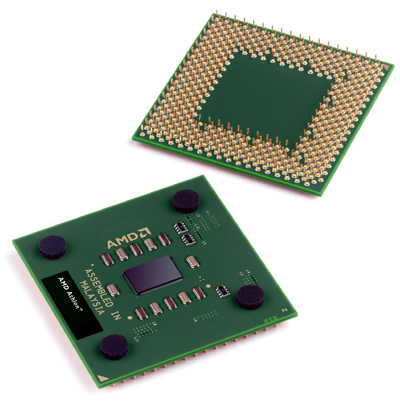
\includegraphics[width=4cm]{Memoria-Cache.jpg}
    \centering
    \caption{Memoria-Cache}
    \label{fig:Memoria-Cache}
    \end{figure}

\subsubsection{Memoria RAM:}

\paragraph{La memoria RAM es el tipo de memoria más importante del computador [...] Esta es un poco menos veloz que la memoria cache pero esta tiene mas capacidad de almacenamiento temporal.La memoria RAM está dividida en celdas en donde sealmacenan temporalmente cada uno de los bits que componen los bytes de la información \cite{taller}}

Fig.\ref{fig:RAM} Memoria RAM
    \begin{figure}[h]
    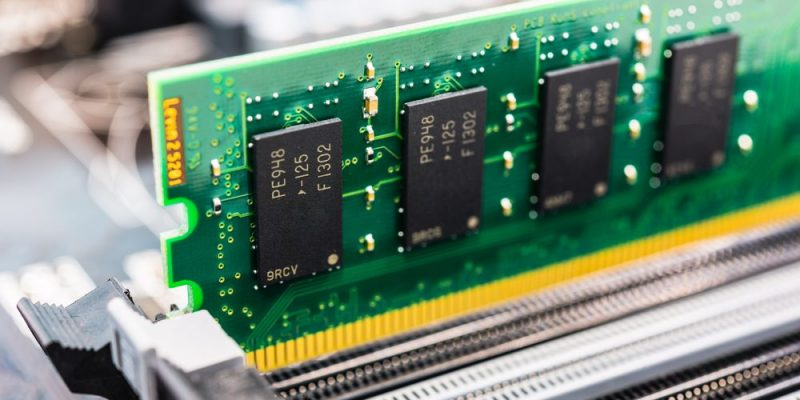
\includegraphics[width=4cm]{RAM.jpg}
    \centering
    \caption{RAM}
    \label{fig:RAM}
    \end{figure}
\subsubsection{Memoria Virtual:}

\paragraph{Esta no es otra cosa más que unaporción del disco duro dedicada exclusivamente a "sostener" temporalmente los pedazos de los
programas y datos en ejecución que se utilizan menos o que ocupan espacio innecesario en
algún momento determinado\cite{taller} }

Fig.\ref{fig:memoria virtual} Memoria Virtual
    \begin{figure}[h]
    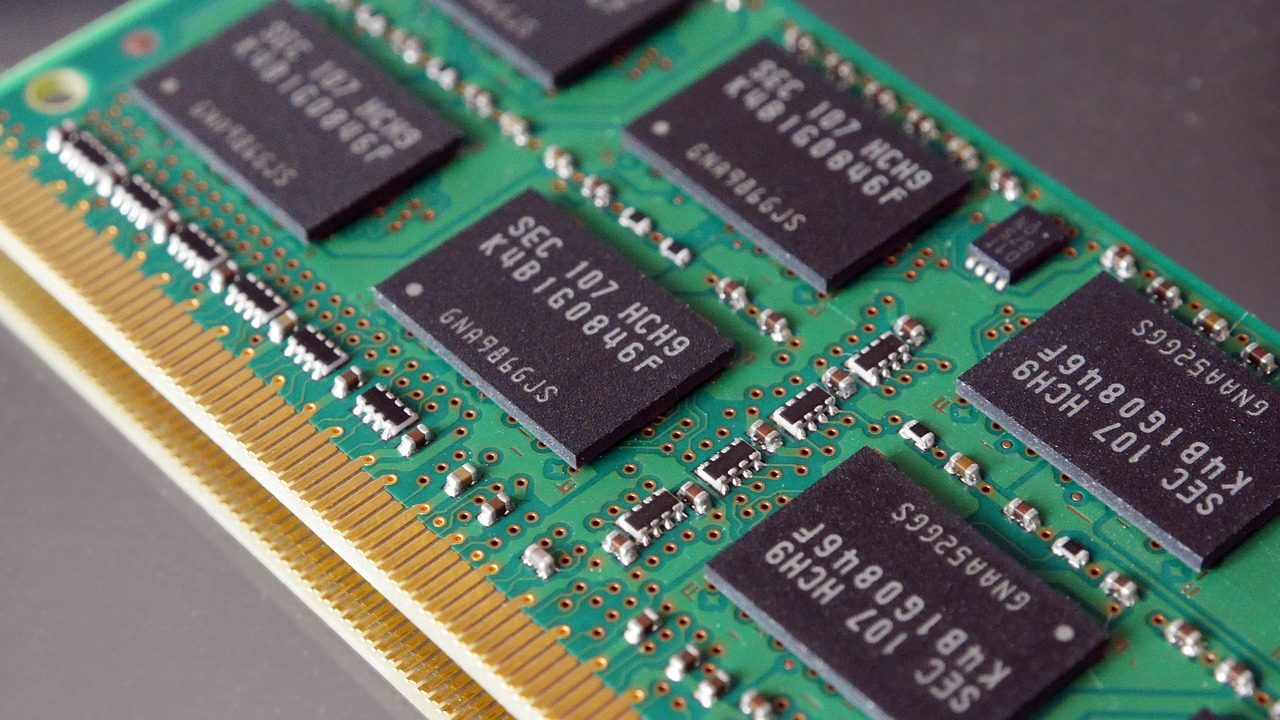
\includegraphics[width=4cm]{memoria virtual.jpg}
    \centering
    \caption{memoria virtual}
    \label{fig:memoria virtual}
    \end{figure}
    
\subsubsection{Disco Duro:}

\paragraph{Esta es la memoria encargada de almacenar todos los programas y datos del computador. es un dispositivo de almacenamiento de datos que emplea un sistema de grabación magnética para almacenar y recuperar archivos digitales.\cite{disco}}

Fig.\ref{fig:disco duro} Disco Duro
    \begin{figure}[h]
    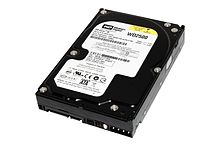
\includegraphics[width=4cm]{disco duro.jpg}
    \centering
    \caption{memoria virtual}
    \label{fig:disco duro}
    \end{figure}
\subsection{Gestión de la memoria}

\paragraph{Supongamos un usuario quiere modificar un documento con un procesador de texto. Para eso abre
un programa, este se encuentra almacenado en el disco duro.Después el microprocesador recibe un aviso de que en una cierta ubicación de la memoria hay una nueva orden y la pasa a buscar. La misma es leída por el microprocesador, indicándole que debe abrir un programa de procesamiento de texto, luego la orden se elimina tanto del procesador como de la memoria,Dicho controlador toma la aplicación, que está almacenada en el disco duro y la lleva hasta la memoria, colocándola en un espacio
vacío de esta para poder trabajar con ella.Una vez que se encuentra cargado en memoria y
funcionando, el usuario envía otra orden con el mouse que le indica al computador que abra
un archivo de texto , el cual también se encuentra almacenado en el disco duro.Luego la busca, se la lleva y la procesa. La misma como ya sabemos, le indica que debe abrir un archivo de texto, A continuación nuestro microprocesador elimina la instrucción ubicada en la memoria para
que no ocupe espacio innecesariamente.Dicho controlador toma el archivo del disco duro y lo transporta hasta la memoria colocándolo en espacios o direcciones vacías de la memoria.Ya en este momento nuestro usuario puede realizar una serie de tareas utilizando las
herramientas del programa, con lo que se harán modificaciones en el documento de
texto abierto. Durante esta instancia de trabajo se darán una infinidad de instrucciones,
procesamientos de datos en el microprocesador así como millones de transferencias de
porciones de datos entre la memoria y el microprocesador, las cuales se irán traduciendo a
texto modificado acorde a las necesidades del usuario.Una vez finalizados los trabajos del usuario con el documento, guardará los cambios. En ese
momento el usuario a través del mouse envía la orden de guardar los cambios. Dicha
instrucción viaja hasta la memoria; a continuación el microprocesador recibe un aviso de
nueva orden; la toma de la memoria, la lee y luego la elimina para que no ocupe espacio
innecesario de la memoria.
 Acto seguido le envía una orden a controlador de memoria, que se encarga de transportar
información de la memoria a otros dispositivos y vice versa a través del bus de datos.Una vez concluidas las tareas, el usuario envía con su mouse la orden de cerrar ,el microprocesador recibe un aviso de orden, la pasa a buscar de su ubicación en memoria,
la lee y luego la elimina para que no ocupe espacio innecesario de la memoria. Dicha
instrucción le ordena que cierre.\cite{taller}}

\subsection{¿Qué hace que una memoria sea más rápida que otra? ¿Por qué esto es importante?}

\paragraph{Una memoria es mas rápido que otra cuando sus discos de rotación dan mas ciclos por segundo en menos tiempo y tambien por el tiempo gastado en el transporte de datos por el bus, esto se ve reflejado en el computador al cargar mas rapido las aplicaciones usadas y ver como obedece el computador de una manera mas veloz cuando uno le da una orden.Esto es muy importante ya que la velocidad nos ayuda a ser mas eficientes a la hora de trabajar con los computadores al poder manejar estos en con mayor velocidad.}

\section{Conclusión} \label{conclulsion}
\paragraph{Podemos concluir de todo lo anteriormente visto que La memoria es una parte esencial en el funcionamiento de muchos elementos electronicos ya que sin este no podria ser posible un buen funcionamiento, tamnbien podemos concluir y hay diferentes tipos de memoria y aunque algunos sean un poco mas lentos que otros todos son totalmente necesarios  para un computador, si faltara alguno de estos se notaria con facilidad.Por ultimo concluimos que afecta la velocidad de la memoria diciendo que es importante su capacidad y el largo del bus por donde se transportan los datos siendo este la comunicacion entre el y otros componentes en el computador. }

\bibliographystyle{IEEEtran}
\bibliography{references}

\end{document}
